% 原书 p.256–p.265（PDF p.264–p.273）
% >>> p264
\section{拉格朗日配边（Lagrangian Cobordism）}

\begin{keytakeaways}
\begin{itemize}
  \item 几何图像：拉格朗日配边是把「若干拉格朗日子流形」与「另一组若干拉格朗日子流形」联系
        起来的、维数高 $1$ 的拉格朗日对象，它比哈密顿动力学更灵活，并可同时处理多个拉格朗日。
  \item 数学工具：拉格朗日悬浮 $S(L,\{\varphi_H^t\}_{t\in\mathbb{R}})$、拉格朗日手术
        $L_1\#_xL_2$、投影 $\pi:V\to\mathbb{R}^2$ 的纤维分析、以及配边范畴
        $\mathrm{Cob}_{\mathrm{Lag}}(M)$。
  \item 本节结论：悬浮与手术分别给出两类基本配边（引理 9.5.1、命题 9.5.1）；
        Biran--Cornea 定理 9.5.1 把配边范畴嵌入一个三角范畴，从而把配边提升为代数信息。
  \item 定量图像：投影像在 $\mathbb{R}^2$ 中的面积给出 $d_s$ 伪度量，它（至少在形式上）小于
        Chekanov--Hofer 度量；「影子」（shadow）则忽略配边投影中的有界洞，用来度量复杂度。
\end{itemize}
\end{keytakeaways}

拉格朗日配边这一概念是为把多个拉格朗日子流形联系起来而引入的。此前，由猜想 5.3.2 我们已经
看到，从（哈密顿）动力学的角度看，拉格朗日子流形之间的关系常常通过它们的相交来反映（这最终
被表述为一个同调理论）。这里，拉格朗日配边有两个优点：(i) 拉格朗日之间的相互作用超出了哈密顿
动力学；(ii) 它使得可以同时讨论多个（特别是多于两个）拉格朗日。

\textbf{拉格朗日悬浮}\quad 为说明拉格朗日配边的来源，让我们从一个简单情形出发。固定拉格朗日子流形 $L\subset(M,\omega)$
与 $(M,\omega)$ 上的哈密顿同痕 $\{\varphi_H^t\}_{t\in[0,1]}$。注意这里的哈密顿函数
$H=H_t$ 只定义在时间区间 $[0,1]$ 上。下面是一个小技巧，可把 $H=H_t$ 延拓到整个 $\R$ 上：
固定光滑函数 $b:[0,1]\to[0,1]$，使得 $b$ 在 $t=0$ 与 $t=1$ 附近为常数，并考虑修改后的同痕
\[
  \{\psi_t\}_{t\in[0,1]}:=\{\varphi_H^{b(t)}\}_{t\in[0,1]};
\]
容易验证 $\{\psi_t\}_{t\in[0,1]}$ 也是哈密顿同痕，由函数
$\widetilde H(t,x)=b'(t)H(b(t),x)$ 对 $(t,x)\in[0,1]\times M$ 生成。特别地，$\widetilde H$
在 $t=0$ 与 $t=1$ 附近为零。

% >>> p265
因此，用 $0$ 延拓之后，就可以在整个 $\R$ 上定义 $\widetilde H$，它生成的动力学与 $H$ 大体相同，
只是时间参数化做了修改。本节中，不失一般性，我们总假定给定的哈密顿同痕
$\{\varphi_H^t\}_{t\in\R}$ 是定义在整个 $\R$ 上的，而相应的哈密顿函数 $H$ 具有紧支撑且支撑在
$(0,1)\times M$ 中。下面的定义是经典的。

\begin{wdefn}{9.5.1}
设 $(M,\omega)$ 为辛流形，$L\subset(M,\omega)$ 为拉格朗日子流形。对哈密顿函数 $H$ 支撑在
$(0,1)\times M$ 中的哈密顿同痕 $\{\varphi_H^t\}_{t\in\R}$，其\textbf{拉格朗日悬浮}
（Lagrangian suspension）定义为
\[
  S\big(L,\{\varphi_H^t\}_{t\in\R}\big)
  :=\big\{(t,H(t,\varphi_H^t(x)),\varphi_H^t(x))\ \big|\ (t,x)\in\R\times L\big\},
\]
它是 $\R^2\times M$ 中的一个子集。
\end{wdefn}

显然，由 $H$ 的定义性质，拉格朗日悬浮在如下意义下是平凡的：
$S(L,\{\varphi_H^t\}_{t\in\R})|_{t\in(-\infty,0]\cup[1,\infty)}=\{(t,0,x)\mid x\in L\}$。
给 $\R^2\times M$ 装备积辛结构 $\omega_{\mathrm{prod}}:=\pi_1^*\omega_{\mathrm{std}}+\pi_2^*\omega$，
则我们有如下结果，它证明了定义 9.5.1 中「拉格朗日悬浮」一词里「拉格朗日」这个形容词是恰当的。

\begin{wlem}{9.5.1}（[180] 中命题 3.1.E）
给定拉格朗日子流形 $L\subset(M,\omega)$ 与哈密顿函数 $H$ 紧支撑在 $(0,1)\times M$ 中的哈密顿
同痕 $\{\varphi_H^t\}_{t\in\R}$，则拉格朗日悬浮 $S(L,\{\varphi_H^t\}_{t\in\R})$ 是
$(\R^2\times M,\omega_{\mathrm{prod}})$ 中的拉格朗日子流形。
\end{wlem}

\begin{wproof}
考虑由下式给出的嵌入 $\Phi:\R\times L\to\R^2\times M$：
\[
  \Phi(t,x)=(t,H(t,\varphi_H^t(x)),\varphi_H^t(x)).
\]
由定义 9.5.1，$\Phi$ 的像恰是拉格朗日悬浮 $S(L,\{\varphi_H^t\}_{t\in\R})$。切向量有两类，
分别由 $\Phi_*(\partial_t)$ 与 $\Phi_*(e)$（对某个 $e\in T_xL$）给出。经计算，我们有
\begin{equation}
  \begin{aligned}
    \Phi_*\left(\frac{\partial}{\partial t}\right)
      &=\left(1,\ \frac{\partial H}{\partial t}+\dd H_t(X_{H_t}),\ X_{H_t}\right),\\
    \Phi_*(e)&=\big(0,\ \dd H_t((\varphi_H^t)_*(e)),\ (\varphi_H^t)_*(e)\big).
  \end{aligned}
  \tag{9.34}
\end{equation}
为证明 $\omega_{\mathrm{prod}}|_{S(L,\{\varphi_H^t\}_{t\in\R})}=0$，等价于证明
$(\Phi^*\omega_{\mathrm{prod}})|_{\R\times L}=0$。分两种情形。

(i) 输入的两个向量是 $\Phi_*(\partial_t)$ 与 $\Phi_*(e)$，即分别来自 $\R$-分量与 $L$-分量。
由 (9.34)，我们有
\[
  \begin{aligned}
    (\Phi^*\omega_{\mathrm{prod}})\left(\frac{\partial}{\partial t},e\right)
    &=(\pi_1^*\omega_{\mathrm{std}}+\pi_2^*\omega)
      \left(\Phi_*\left(\frac{\partial}{\partial t}\right),\Phi_*(e)\right)\\
    &=(\dd t\wedge\dd s)\left(\left(1,\frac{\partial H}{\partial t}\right),
      \big(0,\dd H_t((\varphi_H^t)_*(e))\big)\right)
      +\omega\big(X_{H_t},(\varphi_H^t)_*(e)\big)\\
    &=\dd H_t((\varphi_H^t)_*(e))-\dd H_t((\varphi_H^t)_*(e))=0 .
  \end{aligned}
\]
% >>> p266
(ii) 输入的两个向量是 $\Phi_*(e_1)$ 与 $\Phi_*(e_2)$，即二者都来自 $L$-分量。此时我们有
\[
  \begin{aligned}
    (\Phi^*\omega_{\mathrm{prod}})(e_1,e_2)
    &=(\pi_1^*\omega_{\mathrm{std}}+\pi_2^*\omega)(\Phi_*(e_1),\Phi_*(e_2))\\
    &=\omega\big((\varphi_H^t)_*(e_1),(\varphi_H^t)_*(e_2)\big)
      =\big((\varphi_H^t)^*\omega\big)(e_1,e_2)=0,
  \end{aligned}
\]
其中最后一步用了 $L$ 是拉格朗日的这一条件。
\end{wproof}
% [Tutor Note: 参数化约定的易错点：$\Phi$ 把 $\R\times L$ 的参数 $(t,x)$ 送到三元组
% $(t,H(t,x),\varphi_H^t(x))$，其中第一分量是 $\R^2$ 的「水平」坐标 $t$、第二分量是
% $\R^2$ 的「竖直」坐标 $s$、第三分量在 $M$ 中。因此 (9.34) 中 $\Phi_*(\partial_t)$ 的
% 第二分量是 $\frac{\dd}{\dd t}\big(H(t,\varphi_H^t(x))\big)=H_t$ 的偏导加上
% $\dd H_t(X_{H_t})$（链式法则），第三分量是 $X_{H_t}$。情形 (i) 中 $(\dd t\wedge\dd s)$
% 作用在 $(1,\partial_tH)$ 与 $(0,\dd H_t(\cdot))$ 上得 $\partial_tH\cdot 0$ 与
% $1\cdot\dd H_t(\cdot)$ 之差，即 $\dd H_t((\varphi_H^t)_*(e))$；而
% $\omega(X_{H_t},(\varphi_H^t)_*(e))=-\dd H_t((\varphi_H^t)_*(e))$ 用的是 (1.15) 的
% 符号约定，两项恰好抵消。若把 $\omega$ 的约定换成 $\iota_{X_H}\omega=+\dd H$，此处符号会
% 反过来，故核对时必须与本书 (1.15) 保持一致。情形 (ii) 中第一个因子 $\pi_1^*\omega_{\mathrm{std}}$
% 为零，因为两个向量的 $\R^2$ 分量都为零。]

现在考虑如下投影：$\pi:S(L,\{\varphi_H^t\}_{t\in\R})\subset\R^2\times M\to\R^2$。图 9.9 是
投影的像 $\pi(S(L,\{\varphi_H^t\}_{t\in\R}))\subset\R^2$ 的示意图。

\begin{figure}[htbp]
  \centering
  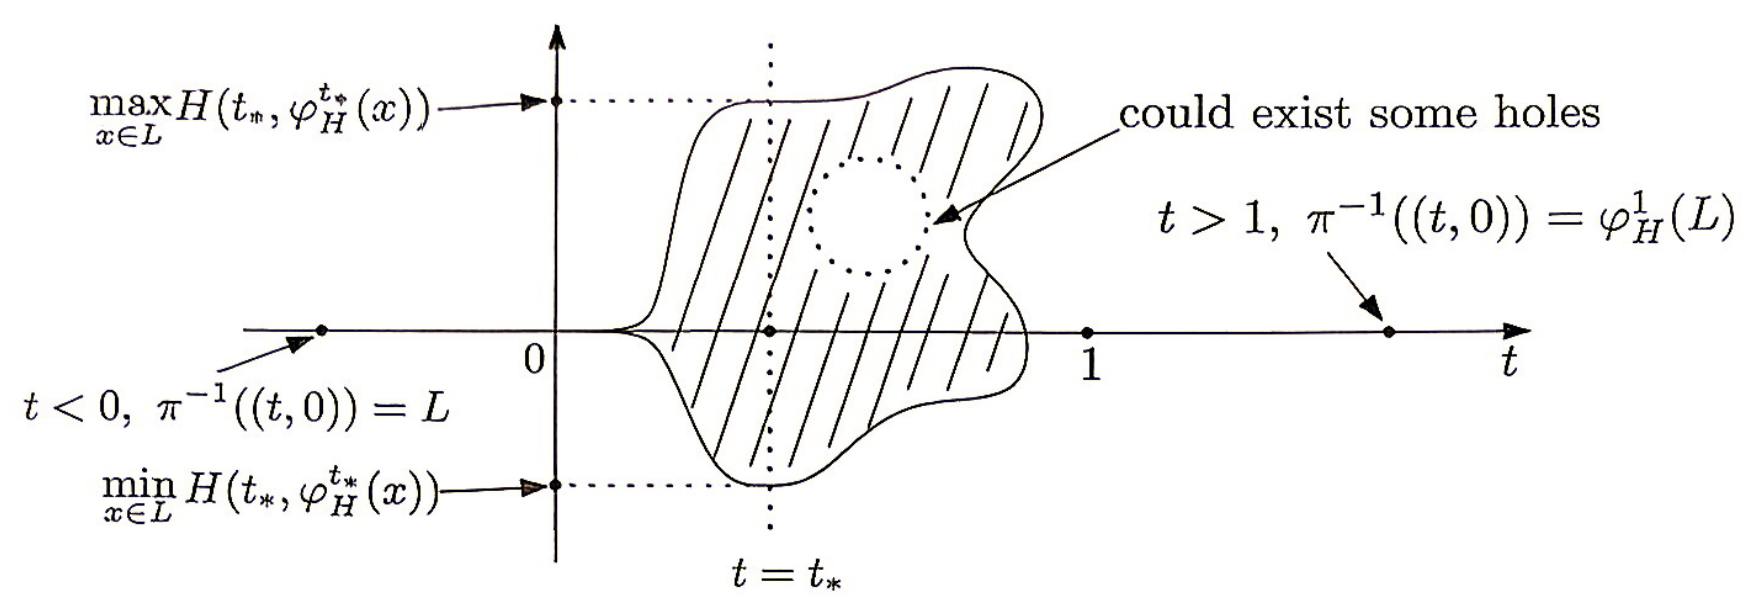
\includegraphics[width=0.85\linewidth]{figures/fig_p266_1.png}
  \caption*{图 9.9\quad $S(L,\{\varphi_H^t\}_{t\in\R})$ 在 $\R^2$ 上的投影示意图
  （原书 p.258, Figure 9.9；PDF p.266）}
\end{figure}

考虑像 $\pi(S(L,\{\varphi_H^t\}_{t\in\R}))\subset\R^2$ 的面积，我们有如下估计
\[
  \Area_{\R^2}\big(\pi(S(L,\{\varphi_H^t\}_{t\in\R}))\big)
  \le\int_0^1\left(\max_{\varphi_H^t(L)}H_t-\min_{\varphi_H^t(L)}H_t\right)\dd t
  \le\|H\|_{\mathrm{Hofer}},
\]
其中 $\|H\|_{\mathrm{Hofer}}$ 表示函数 $H$ 的 Hofer 范数，定义于 (6.1)。相当令人惊讶的是，
这样的几何（来自 $S(L,\{\varphi_H^t\}_{t\in\R})$）与动力学（以
$\|H\|_{\mathrm{Hofer}}$ 衡量）是相关的。

受上面不等式 $\Area(\cdot)\le\|\cdot\|_{\mathrm{Hofer}}$ 的启发，一旦固定了拉格朗日子流形
$L\in(M,\omega)$，人们就可以把另一个量联系到拉格朗日轨道空间
$\mathcal{O}(L)=\{\varphi(L)\mid\varphi\in\Ham(M,\omega)\}$（在 9.3 节中研究）中的元素上。
定义
\[
  d_s(L_1,L_2):=\inf\big\{\Area_{\R^2}\big(\pi(S(L_1,\{\varphi_H^t\}_{t\in\R}))\big)
  \ \big|\ \varphi_H^1(L_1)=L_2\big\}
\]
对任意 $L_1,L_2\in\mathcal{O}(L)$。可以验证 $d_s$ 定义了 $\mathcal{O}(L)$ 上的一个伪度量，
并且它至少在形式意义上小于（或细于）如 (9.20) 中的 Chekanov--Hofer 度量
$\delta_{\mathrm{CH}}(=\delta_{\|\cdot\|_{\mathrm{Hofer}}})$（另见注 9.3.1），后者已在 9.4 节
中讨论过。

回到本节开头，拉格朗日悬浮 $S(L,\{\varphi_H^t\}_{t\in\R})$ 通过空间
$(\R^2\times M,\omega_{\mathrm{prod}})$ 中一个维数高 $1$ 的拉格朗日对象，把两个拉格朗日子流形
$L$ 与 $\varphi_H^1(L)$ 联系起来。从 $\R^2$ 中的投影（即图 9.9）看，除了中间那部分二维

% >>> p267
区域之外，在 $\R^2$ 的一个紧子集之外，投影像由半无限直线组成，其纤维在（负）一端为 $L$，
在（正）一端为 $\varphi_H^1(L)$。

\textbf{拉格朗日手术}\quad 下面这个例子说明多个（多于两个）拉格朗日子流形如何在几何上被联系起来。取两个拉格朗日子流形
$L_1,L_2\subset(M,\omega)$。当它们相交时，在通有位置下交点是点。对单个拉格朗日
$L\subset(M,\omega)$ 的类似情形，$L$ 可以不是嵌入子流形，而可以是带二重交点
（即自交点）的浸入子流形。为说明接下来的故事，让我们考虑如下最简单的局面：
$L_1=\sqrt{-1}\cdot\R\subset\C$ 与 $L_2=\R\subset\C$。它们只在 $0\in\C$ 处相交，为消解这个
交点，我们将在点 $0$ 处施行\emph{拉格朗日手术}。

显式地，取由下式定义的曲线 $\gamma(t):\R\to\C$
\[
  \gamma(t)=
  \begin{cases}
    t & \text{若 } t\le-1,\\
    \sqrt{-1}\cdot t & \text{若 } t\ge1,\\
    a(t)+\sqrt{-1}\cdot b(t) & \text{若 } t\in(-1,1),
  \end{cases}
\]
其中 $a(t),b(t)$ 是 $\R$ 上固定的函数，满足 $a'(t),b'(t)\ge0$，当 $t\ge1$ 时 $a(t)=0$，
当 $t\le-1$ 时 $b(t)=0$，且 $\gamma(t)$ 对 $t\in[0,1]$ 光滑。$\gamma(t)$ 的示意图见图 9.10。
现在考虑 $\C$ 中的如下子集：
\[
  \begin{aligned}
    L_\gamma^1&:=\big\{xa(t)+\sqrt{-1}\cdot xb(t)\in\C\ \big|\ x^2=1,\ x\in\R,\ t\in\R\big\}\\
    &=\{\gamma(t)\}_{t\in[0,1]}\sqcup(-1)\cdot\{\gamma(t)\}_{t\in[0,1]} .
  \end{aligned}
\]
这里记号 $L_\gamma^1$ 中的「$1$」表示 $L_\gamma^1$ 是一维的。在这种低维情形下，

\begin{figure}[htbp]
  \centering
  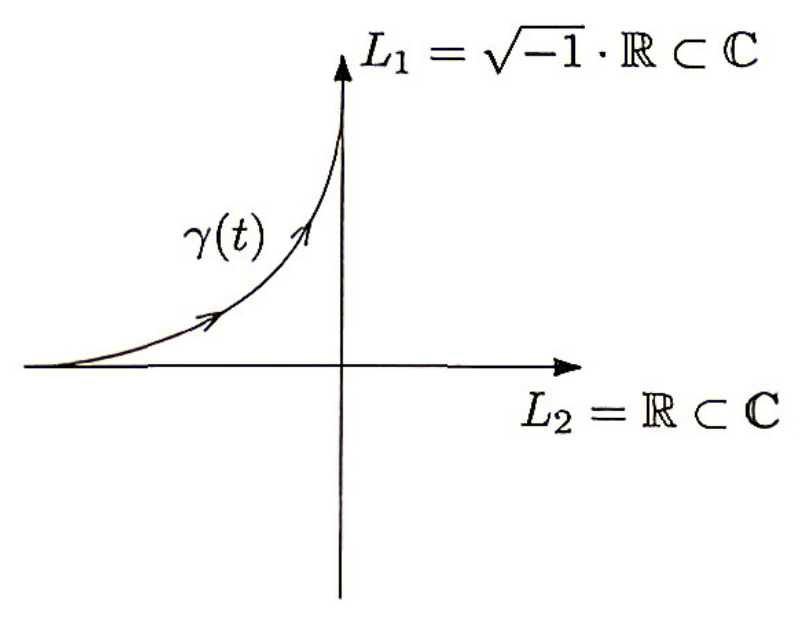
\includegraphics[width=0.42\linewidth]{figures/fig_p267_1.png}
  \caption*{图 9.10\quad 一条参考曲线 $\gamma(t)$（原书 p.259, Figure 9.10；PDF p.267）}
\end{figure}

$L_\gamma^1\subset(\C,\omega_{\mathrm{std}})$ 是拉格朗日子流形，但它分裂成两个连通分支。

模仿上面的构造但置于更高维的情形，对拉格朗日子流形
$L_1=(\sqrt{-1}\cdot\R)^n\subset\C^n$ 与 $L_2=\R^n\subset\C^n$，我们定义
\begin{equation}
  L_\gamma^n:=\left\{(x_1a(t)+\sqrt{-1}\cdot x_1b(t),\cdots,
  x_na(t)+\sqrt{-1}\cdot x_nb(t))\ \middle|\ \sum_{i=1}^nx_i^2=1\right\}
  \tag{9.35}
\end{equation}
% >>> p268
其中 $a(t)$ 与 $b(t)$ 是如上所取的 $\R$ 上的函数。注意原点 $0\in\C^n$ 不再包含在
$L_\gamma^n$ 中。

\begin{wexer}{9.5.1}
证明 (9.35) 中定义的 $L_\gamma^n$ 是 $\C^n$ 中的拉格朗日子流形。
\end{wexer}

我们把这样的 $L_\gamma^n$ 记作 $L_1\#_xL_2$，其中 $x(=0)$ 是 $L_1$ 与 $L_2$ 的交点。
拉格朗日子流形 $L_1\#_xL_2$ 称为 $L_1$ 与 $L_2$ 在交点 $x\in L_1\cap L_2$ 处的
\emph{拉格朗日手术}。

\begin{wrem}{9.5.1}
(i) 对一般的拉格朗日子流形 $L_1,L_2\subset(M,\omega)$，通过辛同胚作局部等同，总能找到
$x\in L_1\cap L_2$ 的一个邻域，使得局部地 $L_1\simeq(\sqrt{-1}\cdot\R)^n$ 且
$L_2\simeq\R^n$。因此 (9.35) 中的构造充当唯一的局部模型。此外，在每个交点充分小的邻域内，
人们可以连续地施行拉格朗日手术，直到不再存在交点。

(ii) 也可以选取另一条对称的曲线 $\gamma^{\mathrm{op}}(t):\R\to\C$，它取值于
$\C(\cong\R^2)$ 的第一象限。与 (9.35) 中相同的拉格朗日手术构造以同样的方式奏效。然而，
我们选择施行手术的顺序或一侧变得至关重要。在图 9.11 中，对一个浸入的拉格朗日子流形 $L$，
我们演示了消解交点的两种方式：选取上面的 $\gamma(t)$，得到的是一个 $S^1$ 的拷贝；而选取对称的
$\gamma^{\mathrm{op}}(t)$，得到的是两个 $S^1$ 的拷贝。
\end{wrem}
% [Tutor Note: 参数化约定——(9.35) 中 $L_\gamma^n$ 由 $\gamma$ 与单位球面
% $S^{n-1}=\{\sum x_i^2=1\}$ 的张成构造：每个 $x\in S^{n-1}$ 给出曲线
% $t\mapsto x\cdot\gamma(t)$，故 $L_\gamma^n$ 是 $\C^n$ 中 $n$ 维实子流形（$\gamma$ 贡献 1 维、
% $S^{n-1}$ 贡献 $n-1$ 维）。$x^2=1$ 即 $x=\pm1$ 正是 $S^0$，因此
% $L_\gamma^1=\{\gamma\}\sqcup\{-\gamma\}$ 的两个分支对应 $\pm1$。注意 $\gamma$ 在
% $t\le-1$ 沿实轴、在 $t\ge1$ 沿虚轴，故 $L_\gamma^n$ 的两端分别渐近于 $L_2=\R^n$ 与
% $L_1=(\sqrt{-1}\R)^n$；这就是手术「把两个拉格朗日接起来」的几何含义。
% 另外，注 (i) 中的 $\simeq$ 应理解为「局部辛同胚意义下等价」，而不是整体同构。]

\begin{figure}[htbp]
  \centering
  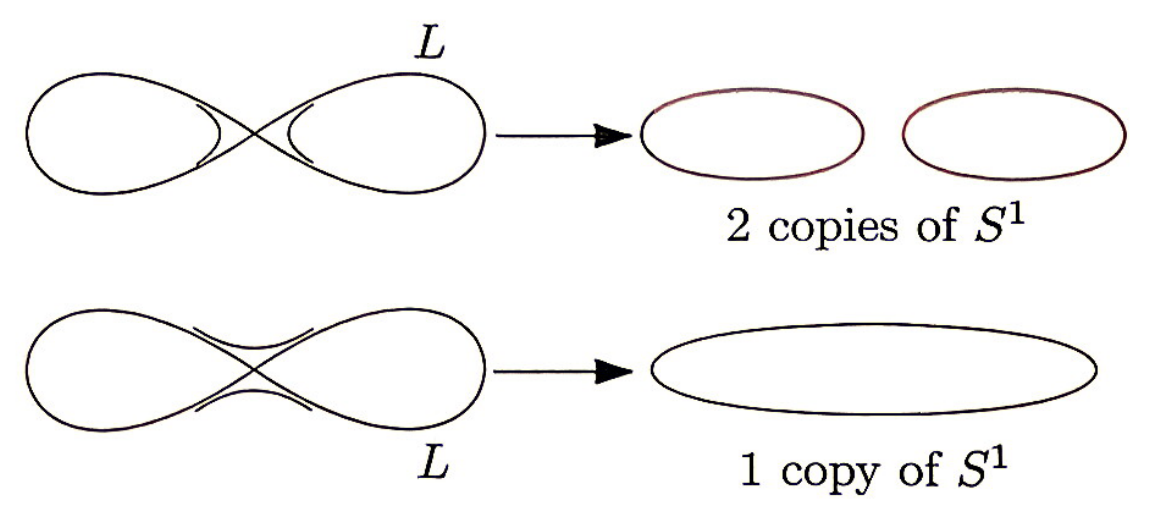
\includegraphics[width=0.72\linewidth]{figures/fig_p268_1.png}
  \caption*{图 9.11\quad 在不同的一侧施行手术得到不同的流形
  （原书 p.260, Figure 9.11；PDF p.268）}
\end{figure}

\begin{wprop}{9.5.1}
给定拉格朗日子流形 $L_1,L_2\in(M^n,\omega)$ 及一个交点 $x\in L_1\cap L_2$，按 (9.35) 施行
拉格朗日手术后，在 $L_1$、$L_2$ 与 $L_1\#_xL_2$ 之间存在一个「配边」。
\end{wprop}

\begin{wproof}
由注 9.5.1，只需在局部模型中考察：$L_1=(\sqrt{-1}\cdot\R)^n$、$L_2=\R^n$ 与 $\C^n$。
为简洁起见，我们考虑 $n=1$，此时同样的论证
% >>> p269
对一般的 $n$ 也适用。定义
\[
  \begin{aligned}
    V_x:={}&\Big(\big\{(x_1a(t)+\sqrt{-1}\cdot x_1b(t),\,
      x_2a(t)+\sqrt{-1}\cdot x_2b(t))\in\C^2\ \big|\ x_1^2+x_2^2=1,\ t\in\R\big\}\Big)\\
    &\cap\Big(\pi^{-1}\big(\{x_1+\sqrt{-1}\cdot y_1\in\C\mid y_1\ge x_1\}\big)\Big),
  \end{aligned}
\]
其中 $\pi:\C^2\to\C$ 是第一个复因子的投影。注意 $V_x$ 的复维数为 $2$（即实维数为 $4$），
而 $L_1\#_xL_2$ 的实维数为 $2$。此外注意 $V_x$ 实际上等于
$L_\gamma^2\cap\pi^{-1}(\{y_1\ge x_1\})$，其中 $L_\gamma^2$ 是由 (9.35) 取 $n=2$ 构造的。
这蕴涵 $V_x$ 是 $\C^2$ 的拉格朗日子流形。

为把 $V_x$ 可视化，让我们把 $V_x$ 投影到第一个 $\C$-分量上，即
$V_x\mapsto x_1a(t)+\sqrt{-1}\cdot x_1b(t)\simeq(x_1a(t),x_1b(t))\in\R^2$
（见图 9.12），然后研究其纤维。有三处不同位置上的纤维特别容易且有趣。

\begin{figure}[htbp]
  \centering
  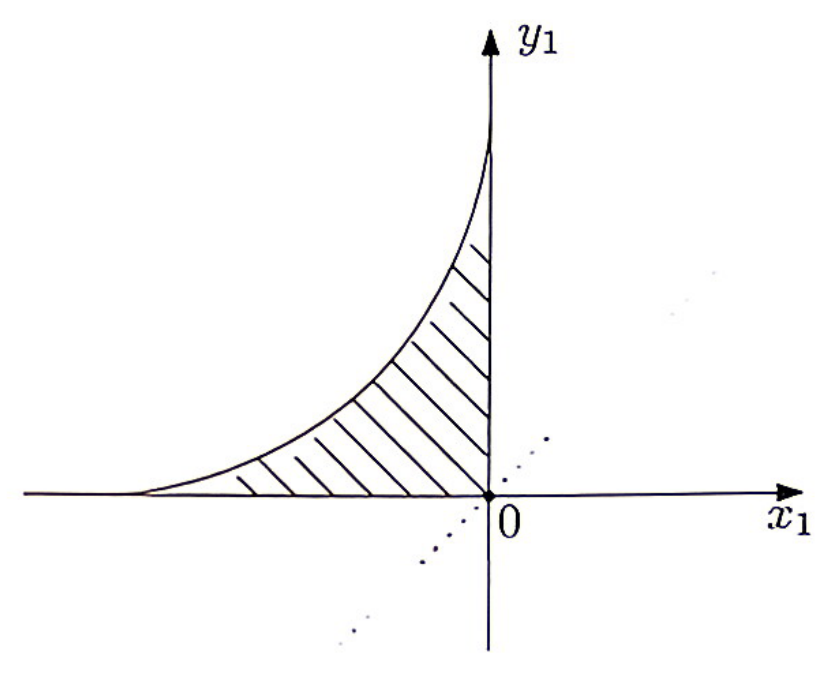
\includegraphics[width=0.45\linewidth]{figures/fig_p269_1.png}
  \caption*{图 9.12\quad $V_x$ 到 $\R^2$ 的投影（原书 p.261, Figure 9.12；PDF p.269）}
\end{figure}

(i) 在投影点 $(x_1a(t),0)$ 之上，其中 $x_1a(t)\le-1$：由于按定义 $a(t)\le0$，我们有
$x_1>0$。同时，由条件 $x_1^2+x_2^2=1$ 知 $x_1\in(0,1]$，这蕴涵 $a(t)\le-1$，从而
$b(t)=0$。因此纤维是
\[
  \pi^{-1}\big((x_1a(t),0)\big)
  =(x_1a(t),0)\times\{x_2a(t)\mid x_2\in[-1,1],\ t\in\R\}
  =(x_1a(t),0)\times L_2,
\]
回忆 $L_2=\R\subset\C$。

(ii) 在投影点 $(0,x_1b(t))$ 之上，其中 $x_1b(t)\ge1$：由于按定义 $b(t)\ge0$，我们有
$x_1>0$。同时，由条件 $x_1^2+x_2^2=1$ 知 $x_1\in(0,1]$，这蕴涵 $b(t)\ge1$，从而
$a(t)=0$。因此纤维是
\[
  \pi^{-1}\big((0,x_1b(t))\big)
  =(0,x_1b(t))\times\{\sqrt{-1}\cdot x_2b(t)\mid x_2\in[-1,1],\ t\in\R\}
  =(0,x_1b(t))\times L_1,
\]
回忆 $L_1=\sqrt{-1}\cdot\R\subset\C$。

% >>> p270
(iii) 在投影点 $(0,0)$ 之上，即 $x_1a(t)=0$ 且 $x_1b(t)=0$：由于 $a(t)$ 与 $b(t)$ 不能
同时为零，我们有 $x_1=0$，由条件 $x_1^2+x_2^2=1$ 这蕴涵 $x_2=\pm1$。因此纤维是
\[
  \pi^{-1}\big((0,0)\big)
  =(0,0)\times\{\pm(a(t)+\sqrt{-1}\cdot b(t))\mid t\in\R\}
  =(0,0)\times L_1\#_xL_2 .
\]
为与纤维 $L_1$、$L_2$ 的构型保持一致，让我们把这个纤维 $L_1\#_xL_2$ 从 $(0,0)$ 手工延拓到
从 $(0,0)$ 出发的整条射线 $y_1=-x_1$ 上。于是我们得到一个多端配边（见图 9.13）。
\end{wproof}

\begin{figure}[htbp]
  \centering
  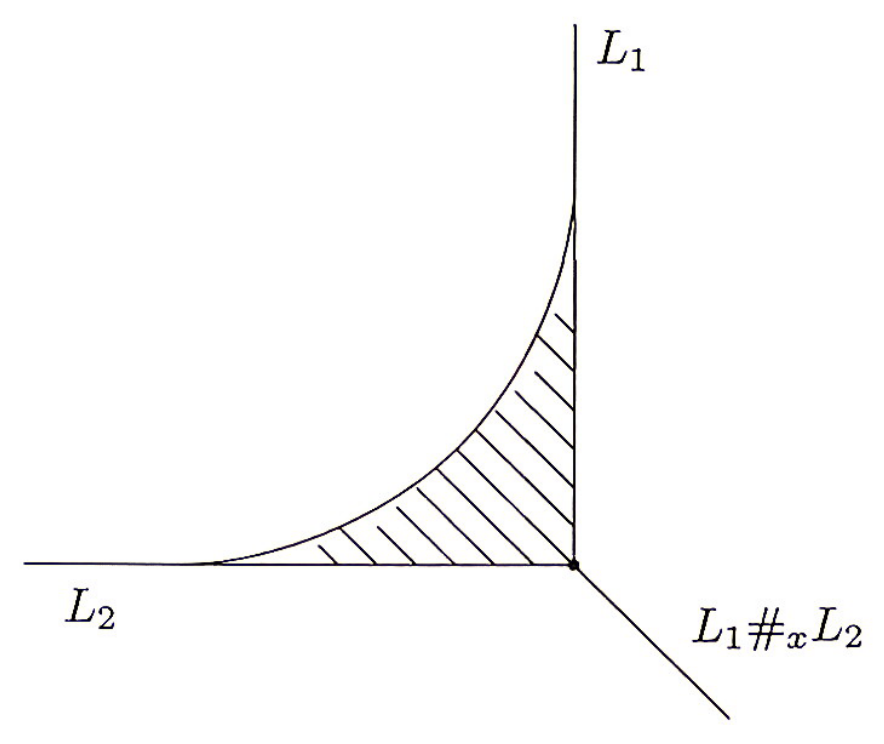
\includegraphics[width=0.45\linewidth]{figures/fig_p270_1.png}
  \caption*{图 9.13\quad 一个多端配边（原书 p.262, Figure 9.13；PDF p.270）}
\end{figure}

\begin{wrem}{9.5.2}
可以基于 $\R$ 上不同的函数 $a(t)$ 与 $b(t)$ 选取不同的曲线 $\gamma(t)$（例如把上面的
$a(t),b(t)$ 作重新标度），使得命题 9.5.1 的证明中 $V_x$ 的投影的阴影部分可以任意小。
\end{wrem}
% [Tutor Note: 本证明是「配边」概念的原型，其要点是：$V_x$ 在 $\C^2$ 中是拉格朗日的，
% 而它在 $\R^2$（第一个 $\C$-因子）上的投影的纤维沿三个「端」分别等于 $L_2$、$L_1$ 与
% $L_1\#_xL_2$。原文最后说「手工延拓到整条射线 $y_1=-x_1$」，这一步并非严格的辛几何构造，
% 而是把纤维方向上的「端」画成射线的绘图约定——真正严格的说法是：$V_x$ 在两个方向上分别
% 收敛到 $\R\times L_2$ 与 $\R\times L_1$，其第三端收敛到 $L_1\#_xL_2$。图中的阴影部分即
% 纤维「被扫过」的区域，其面积正是注 9.5.2 中可任意小的那个量（并对应后文的「影子」）。]

在两处的拉格朗日悬浮与拉格朗日手术中，对给定的（多个）拉格朗日子流形，我们已经看到一些几何
对象——作为维数高 $1$ 的拉格朗日子流形——充当这些给定拉格朗日的配边。下面的定义总结这一现象，
它最初由 P. Biran 与 O. Cornea 引入。

\begin{wdefn}{9.5.2}（[24] 中的定义 2.1.1）
设 $(M,\omega)$ 为辛流形，$(L_1,\cdots,L_k)$ 与 $(L_1',\cdots,L_{k'}')$ 是 $(M,\omega)$ 中
拉格朗日子流形的两个有序组（ordered sets）。一个从 $(L_1,\cdots,L_k)$ 到
$(L_1',\cdots,L_{k'}')$ 的\textbf{拉格朗日配边}（Lagrangian cobordism）是一个拉格朗日子流形
$V\subset(\R^2\times M,\omega_{\mathrm{std}}\oplus\omega)$，满足如下条件：把 $\R^2$ 的坐标记为
$(s,t)$，则存在常数 $R\in\R_{\ge0}$，使得
\begin{enumerate}[label=(\roman*)]
  \item 当 $t\ge R$ 时，投影 $\pi:V\to\R^2$ 的纤维为
  \[
    \bigcup_{i=1}^k\big([R,+\infty)\times\{s=i\}\times L_i\big),
  \]
% >>> p271
        其中 $i\in\R$ 对应于第 $i$ 个拉格朗日子流形 $L_i$；
  \item 当 $t\le-R$ 时，投影 $\pi:V\to\R^2$ 的纤维为
  \[
    \bigcup_{j=1}^{k'}\big((-\infty,-R]\times\{s=j\}\times L_j'\big),
  \]
        其中 $j\in\R$ 对应于第 $j$ 个拉格朗日子流形 $L_j'$。
\end{enumerate}
\end{wdefn}
% [Tutor Note: 原文疑误/记号的简写——这里说「投影 $\pi:V\to\R^2$ 的纤维为
% $\bigcup_i([R,+\infty)\times\{s=i\}\times L_i)$」，严格地说该式给出的是**原像**
% $\pi^{-1}(\{t\ge R\}\cap\bigcup_i\{s=i\})$，而不是单点上的纤维（单点 $(s,t)$ 上的纤维应是
% $L_i$ 或空集）。正确读法：当 $t\ge R$ 时，$\pi(V)\cap\{t\ge R\}=\bigcup_{i=1}^k
% ([R,+\infty)\times\{s=i\})$，且 $\pi^{-1}([R,+\infty)\times\{s=i\})=[R,+\infty)\times
% \{s=i\}\times L_i$。等价地，$V$ 在 $t\ge R$ 的部分恰是若干条半无限「柱」
% $[R,+\infty)\times\{i\}\times L_i$ 的无交并。译文保留原文写法，详见 review_ch09b.md。
% 另注：$(s,t)$ 中 $s$ 是「水平」坐标，$t$ 才是「竖直」的时间/高度坐标，原文有时把两者混称，
% 阅读 Figure 9.14 时以图中标注为准。]

从投影 $\pi(V)\subset\R^2$ 来看，一个拉格朗日配边 $V$ 可以如图 9.14 所示。

\begin{figure}[htbp]
  \centering
  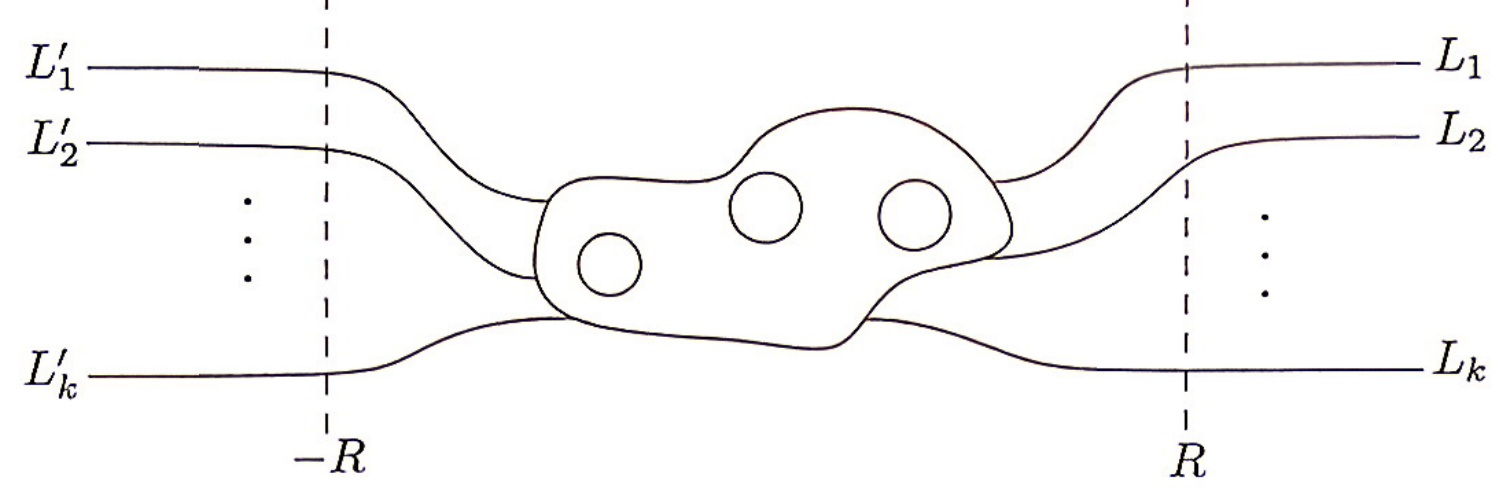
\includegraphics[width=0.85\linewidth]{figures/fig_p271_1.png}
  \caption*{图 9.14\quad 拉格朗日配边 $V$ 的投影 $\pi(V)\subset\R^2$
  （原书 p.263, Figure 9.14；PDF p.271）}
\end{figure}

\begin{wexam}{9.5.1}
(i) 由引理 9.5.1，任何哈密顿函数 $H$ 紧支撑在 $(0,1)\times M$ 中的哈密顿同痕
$\{\varphi_H^t\}_{t\in\R}$ 都生成一个从 $\varphi_H^1(L)$ 到 $L$ 的拉格朗日配边，即拉格朗日
悬浮 $S(L,\{\varphi_H^t\}_{t\in\R})$。

(ii) 给定两个拉格朗日子流形 $L_1,L_2\subset(M,\omega)$ 与一个交点 $x\in L_1\cap L_2$，
命题 9.5.1 蕴涵存在一个从 $L_1\#_xL_2$ 到 $(L_1,L_2)$ 的拉格朗日配边。//
\end{wexam}

\begin{wrem}{9.5.3}
与图 9.9 中的阴影部分类似，对拉格朗日配边 $V\subset(\R^2\times M,\omega_{\mathrm{prod}})$，
其投影在 $(\R^2,\omega_{\mathrm{std}})$ 中有界区域的 $\omega_{\mathrm{std}}$-面积定义了 $V$ 的
一个量，它有助于度量 $V$ 的复杂度。若作如下修改：忽略所有有界洞（即把投影在 $\R^2$-分量上
的洞填满），则这一课题已由 Cornea 与 Shelukhin 在 [57] 中系统研究，所得的量为 $V$ 的
\textbf{影子}（shadow）。
\end{wrem}

\begin{wrem}{9.5.4}
把 $V$ 到 $(\R^2,\omega_{\mathrm{std}})$ 的二维投影约化为一个点，就得到如图 9.15 所示的
投影的简化版本。
\end{wrem}

借用在微分拓扑中配边范畴的概念（例如见 [155]），人们可以用代数的语言重新表述上面演示的
拉格朗日配边。给定辛流形 $(M,\omega)$，如下定义一个范畴 $\mathrm{Cob}_{\mathrm{Lag}}(M)$：
其对象集定义为
\[
  \mathrm{Ob}\big(\mathrm{Cob}_{\mathrm{Lag}}(M)\big)
  :=\{\text{拉格朗日子流形 }L\subset(M,\omega)\},
\]

% >>> p272
\begin{figure}[htbp]
  \centering
  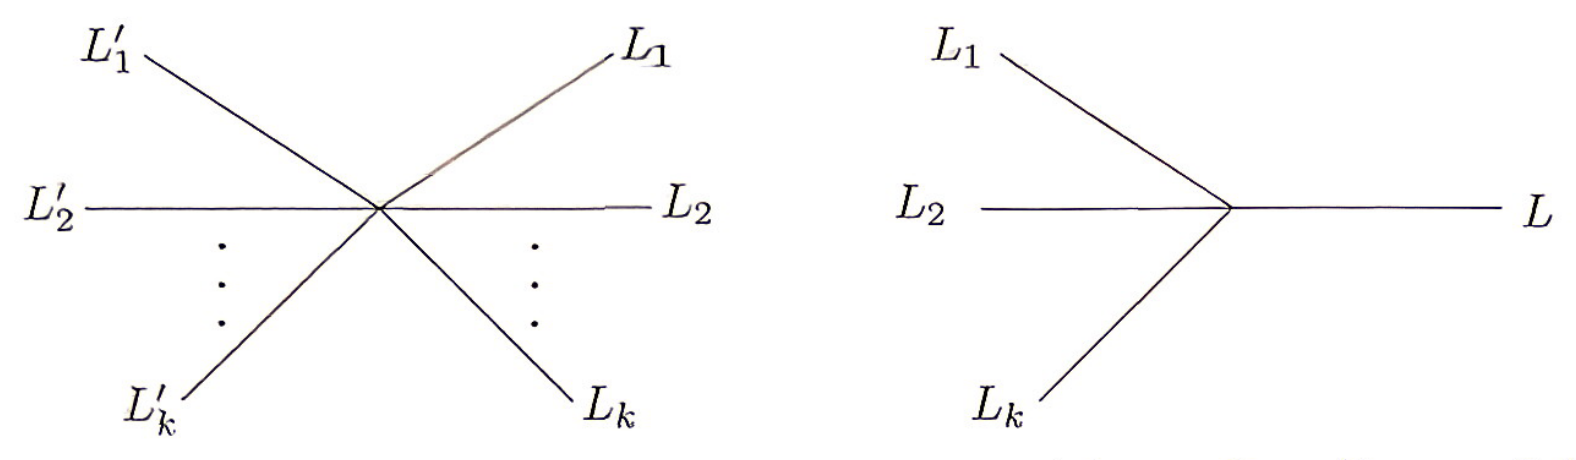
\includegraphics[width=0.85\linewidth]{figures/fig_p272_1.png}
  \caption*{图 9.15\quad 拉格朗日配边的投影的简化版本
  （原书 p.264, Figure 9.15；PDF p.272）}
\end{figure}

而其态射集（或同态集）定义为
\[
  \mathrm{Mor}(L,L'):=
  \left\{V:L\to(L_1,\cdots,L_{k-1},L')\ \middle|\
  \begin{array}{l}
    V\ \text{是一个拉格朗日配边}\\
    L_1,\cdots,L_{k-1}\ \text{都是拉格朗日}
  \end{array}
  \right\}.
\]
注意单位 $\mathbf{1}\in\mathrm{Mor}(L,L)$ 是 $L$ 上的平凡配边，其中
$L_1=\cdots=L_{k-1}=\varnothing$。对任意 $V\in\mathrm{Mor}(L,L')$ 与
$W\in\mathrm{Mor}(L',L'')$，复合 $W\circ V$ 定义为
\[
  W\circ V:L\to(L_1,\cdots,L_k,L_1',\cdots,L_{k'}',L'')\in\mathrm{Mor}(L,L''),
\]
其中我们用第二个拉格朗日配边 $W$ 中出现的拉格朗日子流形替换掉 $L'$。示意图见图 9.16。这个
范畴 $\mathrm{Cob}_{\mathrm{Lag}}(M)$ 称为 $(M,\omega)$ 的\textbf{拉格朗日配边范畴}。

\begin{figure}[htbp]
  \centering
  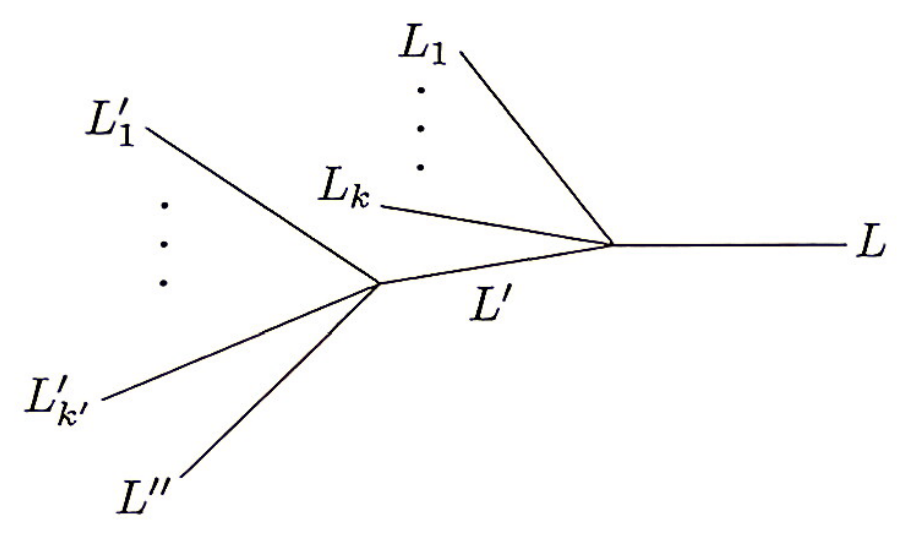
\includegraphics[width=0.55\linewidth]{figures/fig_p272_2.png}
  \caption*{图 9.16\quad $V$ 与 $W$ 的复合（原书 p.264, Figure 9.16；PDF p.272）}
\end{figure}

$\mathrm{Cob}_{\mathrm{Lag}}(M)$ 的定义可以更灵活一些。用
$\widetilde{\mathrm{Cob}}_{\mathrm{Lag}}(M)$ 记另一个范畴，其对象集定义为
\[
  \mathrm{Ob}\big(\widetilde{\mathrm{Cob}}_{\mathrm{Lag}}(M)\big)
  :=\{(L_1,\cdots,L_r)\mid r\in\N,\ L_i\subset(M,\omega)\ \text{对任意 }i\text{ 都是拉格朗日}\};
\]
而其态射集（或同态集）定义为
\[
  \mathrm{Mor}\big((L_1,\cdots,L_r),(K_1,\cdots,K_s)\big)
  :=\left\{W\ \middle|\
  \begin{array}{l}
    W:(K_1,\cdots,K_s)\to(L_1,\cdots,L_r)\ \text{是一个}\\
    \text{如图 9.17 所示的拉格朗日配边}
  \end{array}
  \right\},
\]
% >>> p273
\begin{figure}[htbp]
  \centering
  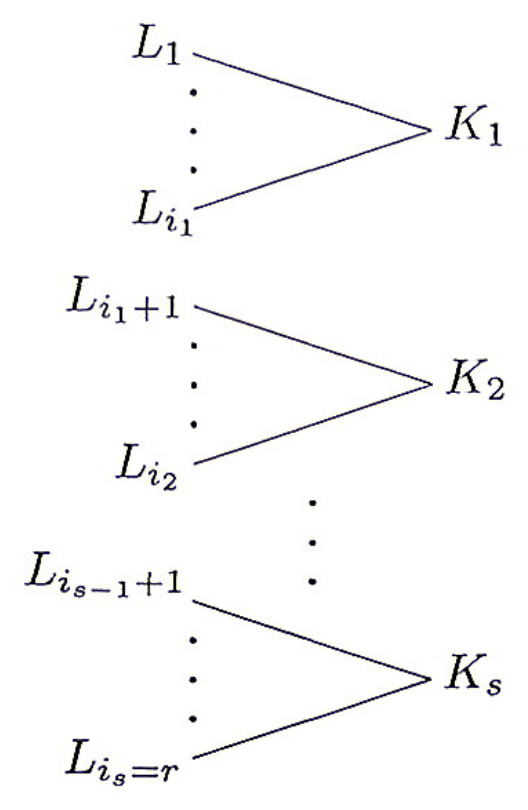
\includegraphics[width=0.36\linewidth]{figures/fig_p273_1.png}
  \caption*{图 9.17\quad 拉格朗日配边 $W$ 的更一般构型
  （原书 p.265, Figure 9.17；PDF p.273）}
\end{figure}

注意在图 9.17 中有一个要求：每个「子配边」的右侧都只有一个端。我们把
$\widetilde{\mathrm{Cob}}_{\mathrm{Lag}}(M)$ 中复合的图示留给有兴趣的读者，鼓励读者自行
给出这一复合的定义。
% [Tutor Note: 这一「只有一个端」的要求是本构造的关键：它保证复合 $W\circ V$ 中每个
% $K_j$ 只被一个子配边「接住」，从而复合后的图形仍是一个合法的配边（否则重合的端会导致
% 纤维不干净、无法定义 $\mathrm{Cob}$ 中的态射）。另外，$\mathrm{Mor}(L,L')$ 的定义里
% 「$L_1\cdots,L_{k-1}$ 都是拉格朗日」这句在原文中缺逗号、且 $k$ 未说明可为零；
% 按上一句「$L_1=\cdots=L_{k-1}=\varnothing$」可知 $k=1$ 时即为平凡配边。]

到目前为止，我们已经从拓扑的表述（即其定义）与范畴的表述这两个角度看到了拉格朗日配边，其中
一切看起来都相当形式化。要进一步推进，就需要在配边范畴 $\mathrm{Cob}_{\mathrm{Lag}}(M)$ 中
引入更多结构。下面是由 Biran 与 Cornea 得到的一个开创性结果，这里我们只陈述一个简略的、
过度简化的版本。完整的陈述见 [24]。

\begin{wthm}{9.5.1}（[25] 中的定理 B）
设 $(M,\omega)$ 为辛流形。则存在一个三角范畴\footnote{三角范畴的定义见 9.6 节。} $\mathcal{F}$，
其对象集 $\mathrm{Ob}(\mathcal{F})$ 由 $(M,\omega)$ 的全部拉格朗日子流形组成，以及一个函子
\[
  \Phi:\mathrm{Cob}_{\mathrm{Lag}}(M)\to\mathcal{F},
\]
使得在对象层面 $\Phi(L)=L$，并且对任意 $V\in\mathrm{Mor}(L,L')$（其中
$V:L\to(L_1,\cdots,L_{k-1},L')$ 对 $(M,\omega)$ 中某些拉格朗日
$L_1,\cdots,L_{k-1}$ 而言），像 $\Phi(V)$ 是一串如下形式的正合三角：
\[
  \left\lbrace
  \begin{array}{l}
    L'\to0\to Z_1\to L'[1]\\
    L_1\to Z_1\to Z_2\to L_2[1]\\
    \cdots\\
    L_{k-2}\to Z_{k-2}\to Z_{k-1}\to L_{k-2}[1]\\
    L_{k-1}\to Z_{k-1}\to L\to L_{k-1}[1]
  \end{array}
  \right.
\]
其中 $Z_1,\cdots,Z_{k-1}$ 是 $\mathrm{Ob}(\mathcal{F})$ 中的某些对象。
\end{wthm}
% [Tutor Note: 这是本节的理论高点：Biran–Cornea 的配边 $\Rightarrow$ 三角范畴的对应，本质上是
% 把 Fukaya 范畴中「拉格朗日配边给出对象的滤过」这一现象公理化。记号说明：
% $L'[1]$ 表示对象 $L'$ 的平移（shift，次数 $+1$），三角范畴中的正合三角形如
% $A\to B\to C\to A[1]$，故上面每一行都是「$L'$（或 $L_i$）→ 锥 → 下一个对象」的迭代。
% 特别是第一行 $L'\to0\to Z_1\to L'[1]$ 意味着 $Z_1\cong L'[1]$（把 $0$ 作为中间项），
% 而最后一行以 $L\to L_{k-1}[1]$ 收尾，正是配边 $V:L\to(L_1,\cdots,L_{k-1},L')$ 的
% 「逐层剥离」结构。作者声明这是过度简化的版本，完整版本（[24] 定理 B）还要求 $\mathcal{F}$
% 满足更多相容性条件，引用时务必以原文为准。]
